\documentclass{article}
\usepackage[english]{babel}
\usepackage[dvips]{graphicx}
\author{A. Soukharev}
\title{Programming implementation of ATLAS EMEC geometry}
\date{27 November 2005}
\begin{document}
\maketitle
\section{Introduction}
This document describes present state of implementation of geometry of ATLAS e/m
endcap calorimeter in Athena framework, namely custom geometric shape
representing
internal EMEC accordion-like structures of absorbers and electrodes.

At the moment of writing the custom shape is used only in Geant4-based
simulation. However, the core class describing EMEC geometry is
Geant4-independent now.

The document's goal is to demonstrate internal algorithms used and
to show meaning of various internal data.

\section{Geometry}
Here is a description of the endcap accordion structures geometry as I
understand it. See \cite{r1, r2, r3, EMEC} for information I'd used.

A single calorimeter endcap consists of two concentric wheels: inner and
outer. These wheels are composed of absorbers and electrodes positioned radially
like spokes. Absorbers and electrodes have a fan-like shape, with the fans 
stretched such that sides are parallel (they are connected to the front and
rear calorimeter surfaces).

Absorbers and electrodes of the same wheel geometrically differ 
only by thickness, so I'll use a common term {\em ``\/fan''} instead
of the words ``absorber'' and ``electrode'' further.

The calorimeter has an axial symmetry, so it is sufficient to set up 
the geometry of a single fan. The fans are positioned with the polar
angle step of $2\pi / n_{fan}\/$, where $n_{fan}\/$ is the number of fans
in a wheel.

The boundary between the inner and outer wheel and the inner radius versus
the inner wheel is angled to
project to the detector center. Thus, while the overall shape of the
endcap is a
disk, the inner and outer wheels are cone-shaped.

For test-beam purposes separate modules were used. Module is $1/8$ part of full
wheel. It has odd number of electrodes (electrode number 0 is removed).

The amplitude of a fan's waves increases with distance from the wheel axis.
Therefore, the wave slant angle $\alpha$ has a complex dependency on the radius.

\begin{figure}
\centering
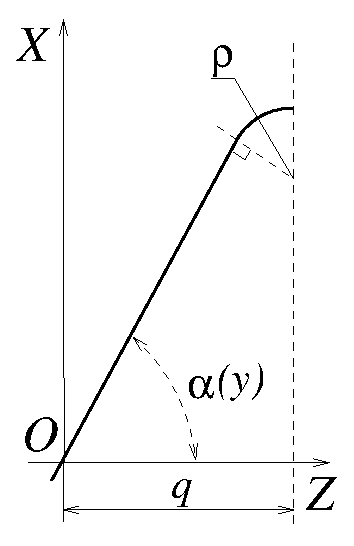
\includegraphics{qwave.eps}
\caption{$1/4\/$ of wave of the fan's neutral fibre. $O$ -- local origin of
coordinates, $q$ -- length of 1/4 of the fan's wave.}
\label{qwave}
\end{figure}


The description of the fan's geometry is based on concept of a {\em neutral
fibre}, defined as a wave-like three-dimensional surface in the middle
of the fan's thickness.

Fig.~\ref{qwave} represents the cross-section of the neutral fibre in the
plane parallel to the plane $OZX$ and displaced from the calorimeter axis
at a distance $y$. There $1/4\/$ of a neutral fibre's wave is shown.
It consists of a straight region, where $x = z \tan \alpha(y)$, and a fold
region. The fold radius $\rho$ does not depend on the distance to the
calorimeter axis.

\begin{figure}
\centering
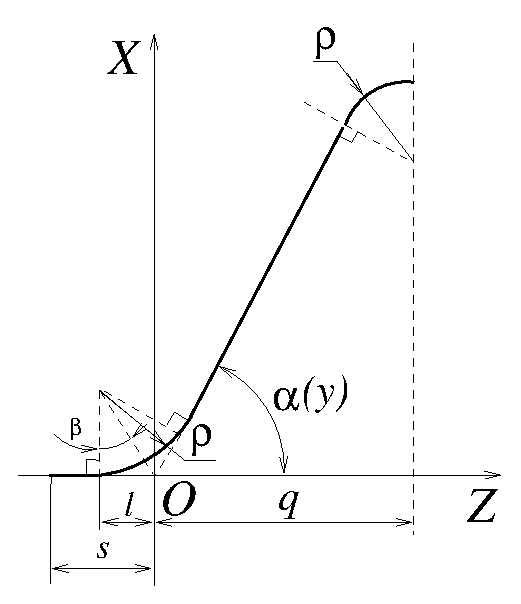
\includegraphics{bqwave.eps}
\caption{$1/4\/$ of the first wave of the fan's neutral fibre. $O$ -- local
origin of coordinates, $q$ -- length of 1/4 of the fan's wave.}
\label{bqwave}
\end{figure}


The geometry of first and last quarter-waves of a fan is a little different
(Fig.~\ref{bqwave}). The fold region that directly connects to the front or rear
wheel surface is of the same radius $\rho$ as a standard wave.
The flat part of the quarter-wave is directed to a point $s\/$ which
is a constant distance from the edge,
so the straight region ($s - l\/$) at the
beginning of the wave varies with $y\/$. The value of $l\/$ is given
by $\rho \tan \beta\/$, where $\beta = \alpha / 2\/$.

All geometrical calculations in the implementation are based on the
computation of the distance to a neutral fibre with the properties described
above.

Sizes are taken from the paper
\cite{geom_tables}. Fan wave slant angle $\alpha$ dependence
on the distance to the calorimeter axis is parameterized with a
polynomial of $4^{th}$ power.

Real absorbers and electrodes consist of several layers, each
layer being made of its own material. In the implementation the multilayer
structure is replaced with a single-layer one using a ``mean'' material.

A concept of a {\em vertical fan} is widely used in the implementation.
Due to the calorimeter's axial symmetry, all the input parameters are
translated to the coordinate system where the fan is positioned along
the $OY\/$ axis. Calculations are conducted in the
coordinate system relative to this fan. If it is
necessary, after the calculation the results are translated back into
the initial coordinate system.

\section{\tt LArWheelCalculator}
Class {\tt LArWheelCalculator} is responsible for neutral fibre's geometry
representation. It is located in {\tt
DetectorDescription/GeoModel/GeoSpecialShapes} package. Unlike older versions,
it is Geant4-independent.

{\bf Important!} Current implementation assumes that each pair of absorbers have
an electrode between them and vice versa. This approach is used
because it significantly improves performance.

Current implementation takes all parameters from DB via {\tt RDBAccessSvc}
service. There are also a lot of hard-coded values which are to be transferred
to DB as well.

\subsection{Data members of {\tt LArWheelCalculator}}
\begin{itemize}
\item {\tt LArWheelCalculator\_t m\_type} --- calculator type (see class
constructor).
\item {\tt int m\_fan\_number} --- internal global variable 
``current fan's number'', may be used
by {\tt get\_sagging} function.
\item {\tt static bool SaggingOn} --- flag to turn sagging on/off.
\item {\tt double sagging\_parameter[5]} --- sagging parameters, actual meaning
is not fixed yet, see {\tt get\_sagging} function.
\item {\tt double slant\_parametrization[5]} --- slant angle $\alpha(y) = a_0 +
a_1y + a_2y^2 + a_3y^3 + a_4y^4$, where $a_0 \div a_4$ --- contents of the
array.
\item {\tt static const double WheelThickness} --- $z$--length of fans.
\item {\tt static double zEMECFrontFace\_value} --- $z$--coordinate of front
face of EMEC.
\item {\tt double StraightStartSection} --- size of starting and
ending fan fold regions ($s$).
\item {\tt double QuarterWaveLength} --- quarter of a fan wave length.
\item {\tt double HalfWaveLength} --- half of a fan wave length.
\item {\tt double FanFoldRadius} --- fold radius ($\rho$).
\item {\tt double ZeroFanPhi} --- polar angle of the fan number zero.
\item {\tt double ZeroFanPhi\_ForDetNeaFan} --- polar angle of the fan number
zero in {\em another type} calculator (see {\tt DistanceToTheNearestFan}
function).
\item {\tt double FanStepOnPhi} --- step on $\varphi$ between fans
($2\pi / n_{fan}$).
\item {\tt int NumberOfWaves} --- number of waves in a fan.
\item {\tt int NumberOfHalfWaves} --- {\tt NumberOfWaves}$ / 2$.
\item {\tt int NumberOfFans} --- number of fans in the wheel ($n_{fan}$).
\item {\tt int HalfNumberOfFans} --- ${\tt NumberOfFans} / 2$.
\item {\tt double FanHalfThickness} --- half of a fan thickness.
\item {\tt int ZeroGapNumber} --- 
constant to convert internal gap number into real.
\item {\tt int FirstFan} --- number of first fan in module.
\item {\tt int LastFan} --- number of last fan in module.
\item {\tt bool isModule} --- true if the calculator is of module type.
\item {\tt bool isElectrode} --- true if the calculator is of electrode type.
\item {\tt bool isInner} --- true if the calculator is of inner wheel or module
type.
\item {\tt float m\_zShift} --- $z$-shift of EMEC.
\item {\tt int m\_AtlasZside} --- not used yet. Used in {\tt
LArWheelEnergyCalculator}.
\end{itemize}

There are also several service data members (DB interface, output).

\subsection{Methods of {\tt LArWheelSolid}}
\begin{itemize}
\item constructor {\tt LArWheelCalculator(LArWheelCalculator\_t type)}\\
Creates calculator of a given {\tt type}. {\tt type} is enumerated constant,
one of {\tt LArWheelCalculator::LArWheelCalculator\_t InnerAbsorberWheel},
{\tt InnerElectrodWheel}, {\tt InnerAbsorberModule}, {\tt InnerElectrodModule},
{\tt OuterAbsorberWheel}, {\tt OuterElectrodWheel}, {\tt OuterAbsorberModule},
{\tt OuterElectrodModule}. Some parts of initialization are separated to
functions {\tt void inner\_wheel\_init(void)}, {\tt void
outer\_wheel\_init(void)}, {\tt void module\_init(void)}.

\item {\tt static const char *LArWheelCalculatorTypeString((LArWheelCalculator\_t type)}\\
Converts {\tt type} to its text representation.

\item {\tt dobule parameterized\_slant\_angle(double r)}\\
Returns wave slant angle $\alpha$ [radian] for a given radius $r$ [mm].

\item {\tt doube DistanceToTheNeutralFibre(const Hep3Vector \&p) const}\\
Returns the shortest distance from the point $p$ to the neutral fibre of the
vertical fan. The returned value is positive if $p$ is in
the region of relatively greater polar angle to the neutral fibre, and negative
otherwise.

The function works in a 2-dimensional approximation.
The calculations are made in the plane parallel to plane $OZX$ and going through
the point $p$, $p_y$ is used to get slant angle. The routine makes use of the
symmetry of waves of the
neutral fibre about the ``knot'' (the point of inflection at $O$ in
Fig.~\ref{qwave}).

If sagging is on, $p_x$ is summed up with the value returned by {\tt
get\_sagging(p)}. This simulates corresponding deformation of the neutral fibre
in the opposite direction \cite{p3}.

Using $p_z$ the function determines the quarter-wave of the
neutral fibre nearest to $p$. If this is neither the first nor the last
quarter-wave, the coordinates $(p_z, p_x)$ are transformed in the following way:
\begin{enumerate}
\item  a shift on $z$ is performed, so the local coordinate origin
$O$ is moved to the knot point,
\item odd half-waves are mirrored relatively to local $OZ$ axis,
\item odd quarter-waves are additionally inverted relative to
local coordinate origin $O$.
\end{enumerate}

After these transformations, all the initial cases are moved into a
standard coordinate system: the nearest quarter-wave where
local coordinates $z$ and $x$ are positive (Fig.~\ref{qwave}).

\begin{figure}
\centering
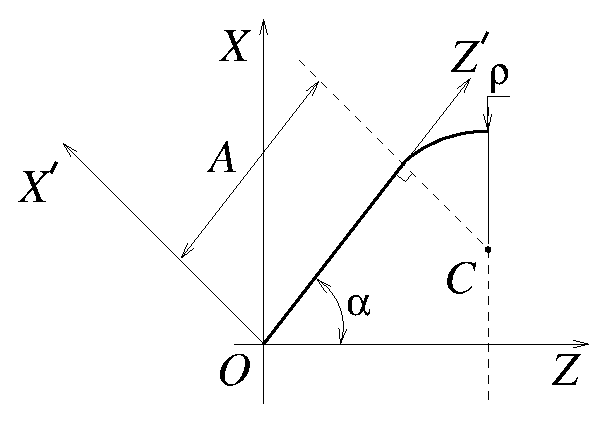
\includegraphics{qwave_prime.eps}
\caption{Calculation of distance $d$ from point $(z, x)$ to neutral fibre. 
If $z^{\prime}< A\/$, then  $d=x^{\prime}\/$, else $d =
\sqrt{(x^{\prime}-A)^2 + (z^{\prime}+\rho)^2} - \rho\/$.}
\label{qwave_prime}
\end{figure}


Next, the local coordinate system is rotated so the straight part of the quarter-wave
is positioned along the $Z^{\prime}$ axis (Fig.~\ref{qwave_prime}).
In this coordinate system it is easy to determine if the initial point is
nearer to
the straight part of the quarter-wave or to the fold region. In both cases the
distance is computed using simple exact two-dimensional formulas.

At the end the result is given with the correct sign, depending on
which transformations were performed.

\begin{figure}
\centering
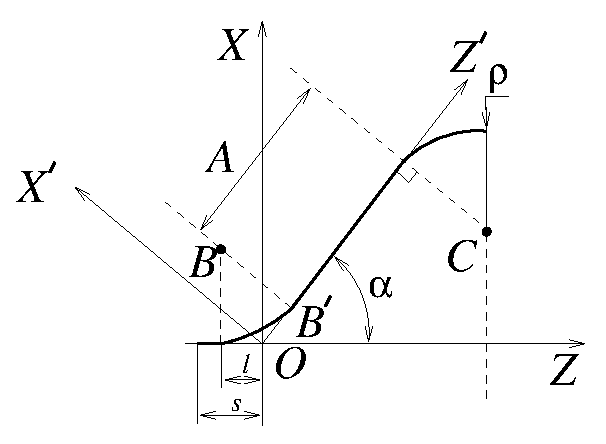
\includegraphics{bqwave_prime.eps}
\caption{Calculation of the distance $d$ from point $(z, x)$ to the
fan's neutral fibre, in the case of the starting quarter-wave.
If $z < -l\/$ and the input point is below the $BB^{\prime}\/$ line, then $d = x$.
If $z^{\prime} < l\/$, then $d =
\sqrt{(x^{\prime}-\rho)^2 + (z^{\prime}-l)^2} - 
\rho\/$, if $z^{\prime}< A\/$, then  $d=x^{\prime}\/$,
else $d = \sqrt{(x^{\prime} + \rho)^2 +
(z^{\prime}-(A + l))^2} - \rho\/$. } 
\label{bqwave_prime}
\end{figure}


In the case of first and last quarter-waves the situation becomes more complex
due to
the existence of the additional fold region.
Using symmetry the last quarter-wave is transformed to the first one.
The next steps are almost the same as the ones for the regular quarter-wave;
the only
exception is that the local coordinate origin is positioned while transforming, not
into
the beginning of the quarter-wave, but into the cross point of the straight part
that continues into the local $OZ$ axis (Fig.~\ref{bqwave_prime}). 

\item {\tt Hep3Vector NearestPointOnNeutralFibre(const Hep3Vector \&p) const}\\
This function is nearly identical to the function {\tt
DistanceToTheNeutralFibre}
and uses the same technique.
 The function returns the point on the
vertical fan neutral fibre which is the ``nearest'' to $p$ as defined by
{\tt DistanceToTheNeutralFibre}.

\item {\tt double DistanceToTheNearestFan(Hep3Vector \&p)}\\
First the function determines the fan nearest to the given point.
It searches for a pair of fans of {\em another type} (i. e. {\em electrodes},
if the calculator is for {\em absorbers}, and vice versa)
containing the point between them using the following algorithm.
First of all, using the formula
\[i = \mbox{int}((p_{\varphi} - \pi/2 - {\tt ZeroFanPhi\_ForDetNeaFan}) /
{\tt FanStepOnPhi})\] 
the number of one of the nearest-to-the-point fans is determined.
Next, the neighboring fans are checked one by one until the fan's pair will be
found where the distance from $p$ to the neutral fibre of the first fan of the
pair is positive and the distance to the second one is negative.
That means that $p$ is located between the fans of this pair. There is a fan
of current type between them which is the nearest one to the point $p$.
{\tt m\_fan\_number} is set to number of the nearest fan.

For module-type calculators, $\varphi$-edges of the module are properly
accounted for.

Returns distance to the nearest
fan's neutral fibre. Input vector $p$ is rotated to the vertical fan's
coordinate system.

\item {\tt std::pair<int, int> GetPhiGapAndSide(const Hep3Vector \&p)}\\
Follows similar to {\tt DistanceToTheNearestFan()} algorithm to find the gap
containing the input point. Number of this gap is the number of the fan of {\em
another type} as well and it is returned as a first member of pair. Second
member is 
either $-1$ if the point is closer to the fan located at less $\varphi$ or $1$
if it is closer to the greater-$\varphi$ fan.

The function affects {\tt m\_fan\_number}.

\item {\tt int GetPhiGap(const Hep3Vector \&p)}\\
This is a shortcut to {\tt GetPhiGapAndSide(p).first}.

\item {\tt double get\_sagging(const Hep3Vector \&p) const}\\
The function returns sagging value for given point $p$ in vertical fan's
coordinate system. {\tt m\_fan\_number} could be used to introduce dependence on
fan number. Function used to calculate sagging value should be smooth.
Apparently it will being tuned later.

\item {\tt int PhiGapNumberForWheel(int) const}\\
Converts gap number in module into gap number in wheel.

\item There are also a lot of {\tt Get}-functions for data members, see class
description in the header file.

\end{itemize}

\section{\tt LArWheelSolid}
{\tt LArWheelSolid} is a custom Geant4 solid. The class is located in
{\tt Simulation/G4Utilities/Geo2G4} package. There is exact copy of the class in
{\tt LArCalorimeter/LArG4/LArG4EC} package; it will disappear as soon as
possible.

Now {\tt LArWheelSolid} has an option to represent a module instead of a wheel.

To do: to make the class use {\tt MsgStream} and database services.

\subsection{Geant4 requirements}
In the Geant4 package a solid is a class; when you create a new type of solid
it must be inherited from the base class {\tt G4VSolid} and the following
methods must be implemented \cite{G4VSolid}:
\begin{itemize}
\item {\tt Inside($\vec{p}\/$)} --- determines if the point $p$ 
is inside of solid, on its surface, or outside.
\item {\tt DistanceToIn($\vec{p}\/$), DistanceToOut($\vec{p}\/$)} 
--- determines the shortest distance from the point $p$ 
located outside or inside of the solid (respectively) to the solid surface.
\item {\tt SurfaceNormal($\vec{p}\/$)} --- 
determines a vector normal to the solid surface and going through the point
$p$. 
\item {\tt DistanceToIn$(\vec{p}, \vec{v})$}, 
{\tt DistanceToOut$(\vec{p}, \vec{v})$} --- compute the distance
from the point $p$ located outside or inside of the solid (respectively)
to the solid surface along the arbitrary vector $\vec{v}\/$.
\item {\tt GetEntityType}, {\tt DescribeYourselfTo}, {\tt GetExtent},
{\tt CreatePolyhedron}, 
{\tt CreateNURBS} --- special functions for tracking and solid drawing.
\end{itemize}

One important thing which I encountered is the following: the information
given by the functions mentioned above must be self-consistent. For
example, if {\tt DistanceToIn$(\vec{p}, \vec{v})$} returns value $d$ then
{\tt Inside($\vec{p} + d |\vec{v}|)$} should not return ``outside''. Otherwise
the Geant4 tracking algorithm may enter into an infinite loop at the solid
surface.

\subsection{List of data members of {\tt LArWheelSolid}}
\begin{itemize}
\item {\tt LArWheelSolid\_t Type} --- wheel type (see constructor).
\item {\tt LArWheelCalculator *Calculator} --- pointer to calculator object.
\item {\tt G4double FanHalfThickness} --- half of a fan thickness.
\item {\tt FanPhiAmplitude} --- polar angle half-size of a fan plus some safety
pad.
\item {\tt static const G4double Tolerance} --- precision of solid boundary
determination (see Geant4 documentation for determination of surface of a
solid).
\item {\tt static const G4double IterationPrecision} --- precision required to
stop iterations.
\item {\tt static const G4double IterationPrecision2} --- second power of
{\tt IterationPrecision}. 
\item {\tt static const unsigned int IterationsLimit} --- maximal number of
iterations; required to avoid infinite loops in case of some error.
\item {\tt G4Polycone *BoundingPolycone} --- an object of class {\tt
G4Polycone}, which represents 
a solid's boundary surface. It helps to process easily the points which are
certainly outside of the solid. It is also used to represent the solid for 
some Geant4 special functions. In case of module this is a polycone sector.

\item {\tt G4Polycone **FanSection}, {\tt G4int MaxFanSection},
{\tt G4double *FanSectionLimits}, {\tt G4int MaxFanSectionLimits} ---
array {\tt FanSection} contains objects of type {\tt G4Polycone}
corresponding to sections of the vertical fan.
{\tt FanSection[i]} is a polyconical sector containing a
half-wave of the vertical fan. First and last quarter-waves have two fan
sections, for the starting/finishing fold region and for the rest of the
quarter-wave separately. $Z$-boundaries of fan sections 
are also stored in the array {\tt FanSectionLimits}. Data members
{\tt MaxFanSection} and {\tt MaxFanSectionLimits} contain the maximum (for a
given wheel type) numbers of fan sections and their edges correspondingly.

The polar angle size of a fan section is enough to capture all the points 
between the vertical fan and its nearest neighbors.

The {\tt FanSection[i]} objects are used by the functions that calculate the
distance to the solid surface along an arbitrary vector.
\item {\tt G4double MinPhi}, {\tt G4double MaxPhi} --- $\varphi$-boundaries
of {\tt BoundingPolycone}, {\tt G4double PhiPosition} --- its orientation. (Used
for module-type solid only.)
\item {\tt G4bool Verbose} --- unused. Will be dropped later.
\end{itemize}

\subsection{Methods of {\tt LArWheelSolid}}
\begin{itemize}
\item Constructor {\tt LArWheelSolid(const G4String \&name, LArWheelSolid\_t
type)}\\
{\tt LArSolidWheel\_t} is an enumerator type, defined values are
{\tt InnerAbsorberWheel},
{\tt InnerElectrodWheel}, {\tt InnerAbsorberModule}, {\tt InnerElectrodModule},
{\tt OuterAbsorberWheel}, {\tt OuterElectrodWheel}, {\tt OuterAbsorberModule},
{\tt OuterElectrodModule}. {\tt name} is solid name.

It is assumed that physical volumes made of each type of solid will be
positioned at a common place (at the vector $(0, 0, Z_0)$) without rotation (or
with the same rotation if it is necessary). If so, the relative
positions  will be correct: electrodes between absorbers of the corresponding
wheel, the outer wheel surrounds the inner one (and similar for modules).

Constructor creates {\tt LArWheelCalculator} object of corresponding type.

Functions {\tt inner\_solid\_init}, {\tt outer\_solid\_init} and {\tt
set\_phi\_size} are also used by the constructor.

\item {\tt Inside$(\vec{p})$}\\
This function checks if the point $p$ is inside of the {\tt BoundingPolycone}.
If it is, then it determines the distance to the nearest-to-$p$ fan and 
checks if the
point is inside or on the surface (comparing the distance with {\tt
HalfFanThickness}).

\item {\tt DistanceToIn$(\vec{p})$}\\
The function checks if the point $p$ is not outside of the {\tt
BoundingPolycone}. If yes, then it determines the distance to the nearest-to-$p$
fan's neutral fibre and subtracts {\tt HalfFanThickness}. Otherwise it 
passes $p$ to the {\tt DistanceToIn$(\vec{p})$} method of {\tt
BoundingPolycone}.

\item {\tt DistanceToOut$(\vec{p})$}\\
The function checks if the point $p$ is not outside of the {\tt
BoundingPolycone}. If 
yes, then it determines the distance to the nearest fan's neutral fibre,
calculates the distance to the fan's surface, compares it with the distance to
the {\tt BoundingPolycone}'s surface and returns the smaller one. If the point
is not inside of the fan or it is outside of the {\tt BoundingPolycone} the
function returns zero.

\item {\tt SurfaceNormal$(\vec{p})$}\\
The function checks if the point $p$ is inside the {\tt BoundingPolycone}. If
yes, then it determines the nearest fan, finds the nearest point on the fan's
neutral fibre and returns the unit vector pointing to $p$ from this point.
Otherwise it 
passes $p$ to the {\tt SurfaceNormal$(\vec{p})$} method of {\tt
BoundingPolycone}.

\item {\tt out\_iteration\_process$(\vec{p}, \vec{q})$}\\
This function searches for the exit point of segment $pq$ from the fan's
half-wave in the event that $q$ is not inside the fan. The points $p$ and $q$
should be in the same {\tt FanSection}.

The function uses an iterative technique of dividing a segment in half.
At the $i\/$th step 
\[\vec{p}_{i+1} = \frac{\vec{p}_i+\vec{q}_i}{2}, \vec{q}_{i+1} = \vec{q}_i,\]
if the point $\frac{\vec{p}_i+\vec{q}_i}{2}$ is not outside the fan, and
\[\vec{p}_{i+1} = \vec{p}_i,  \vec{q}_{i+1} = \frac{\vec{p}_i+\vec{q}_i}{2},\]
otherwise. The process stops when
$|\vec{p}_i-\vec{q}_i|<{\tt IterationPrecision\/}\/$ or $i$ has reached the {\tt
IterationsLimit}.

\begin{figure}
\centering
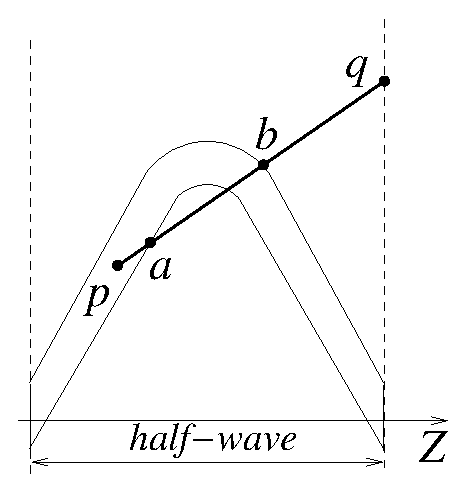
\includegraphics[width=0.33\textwidth,height=0.4\textwidth]{out_iter.eps}
\caption{}
\label{out_iter}
\end{figure}

When a situation is like that shown in Fig.~\ref{out_iter}, 
the function may either find point $a$ or point $b$. It is up to the user to
spot the potential ambiguity and call this function again.

The function returns the distance from the point $p$ to one of the exiting
points. The exiting point is not inside the fan.
 
\item {\tt search\_for\_most\_remoted\_point$(\vec{p}, \vec{q}, \vec{r})$}\\
This function searches on the segment $pq$ for the point which is the
most distant from the neutral fibre of the vertical fan and sets
vector $r$ to it. It also returns a boolean value which is true if
during the search a point outside the vertical fan is encountered
(this allows us to apply {\tt out\_iteration\_process$(\vec{p},
\vec{r})$} here) or false if $pq$ is completely inside the vertical
fan (in this case $r$ is useless). The points $p$ and $q$ should be in
the same {\tt FanSection}.

Next there is a search for the most distant point of segment
$pq$ from the neutral fibre. The search is performed by successively 
dividing the segment in half and looking for the point
where second power of the distance $d$
from segment $pq$ to the neutral fibre is maximal.
At the $i\/$th step 
\[ \vec{p}_{i+1} = \frac{\vec{p}_i+\vec{q}_i}{2}, \vec{q}_{i+1} = \vec{q}_i,\]
if the sign of the derivative $(d^2)^{\prime}$ in the point
$\frac{\vec{p}_i+\vec{q}_i}{2}$ is positive and 
\[\vec{p}_{i+1} = \vec{p}_i, \vec{q}_{i+1} = \frac{\vec{p}_i+\vec{q}_i}{2},\]
otherwise. 
The sign of $(d^2)^{\prime}$ is defined as the sign of the expression
\[d^2(\frac{\vec{p}_i+\vec{q}_i}{2}) -
d^2(\frac{\vec{p}_i+\vec{q}_i}{2}-\vec{\delta})\/,\] where \[\vec{\delta} =
\frac{\vec{q}-\vec{p}}{|\vec{q}-\vec{p}|}\times{\tt IterationPrecision}\] is
small vector along the segment $pq$.
The process is stopped when 
$|\vec{p}_i-\vec{q}_i|<{\tt IterationPrecision}$ or $i$ has reached the {\tt
IterationsLimit\/}. The process is stopped prematurely if the point
$\frac{\vec{p}_i+\vec{q}_i}{2}$ is situated outside of the fan.

If the process has not been stopped prematurely that means the whole segment
$pq$ is inside the current half-wave of the fan.

\item {\tt distance\_to\_out$(\vec{p}, \vec{v})$}\\
This function calculates the distance along the vector
$\vec{v}$ from the point $p$ to the surface of the vertical fan. $\vec{v}$
should be a unit vector. 

First, the function determines in which {\tt FanSection} the point $p$
is located and finds point $a$, the exit point of the line
$\vec{p}+\vec{v}t$ out of the {\tt FanSection}. 
If $a$ is outside of the vertical fan then the function\\ 
{\tt out\_iteration\_process} is called and the line's exit point $q$ out of
the fan is found. Due tothe  potential ambiguity 
of the {\tt out\_iteration\_process} result, it is
not safe to assume that the point $q$ is the nearest exit point.
If the point $a$
is positioned inside the fan then $q$ is set equal to $a$.

Next there is a search for the most distant point of segment
$pq$ from the neutral fibre.
If there is a point outside the vertical fan on $pq$, then a
new {\tt out\_iteration\_process} is called and its result is returned.

If the point $q$ has been found
earlier by the function {\tt out\_iteration\_process} then $q$ is the point
desired, and the function returns the length of the segment $pq$. Otherwise the
search for the exit point is performed in the neighbor half-wave of the fan
in the direction of the segment $pq$.
The search transition is not performed if $pq$ is directed beyond the beginning of the
first half-wave or beyond the end of last half-wave of the fan. In that case the
function returns the length of the segment $pq$.

Due to the properties of the geometry the search for the exiting point in the
neighbor half-wave could sometimes be simplified.

\item {\tt DistanceToOut$(\vec{p}, \vec{v}, \dots)$}\\
This function checks if the point $p$ is inside of the {\tt BoundingPolycone}. If
yes, then it determines inside of which fan the point $p$ is positioned and
returns the distance to the fan's surface along the vector $\vec{v}$. If the
point $p$ is not inside of any fan or outside of the
{\tt BoundingPolycone}, zero is returned.

The function has three more parameters, which are substituted by ``\dots'' in
the header. These parameters are {\tt G4bool calcNorm}, {\tt G4bool *ValidNorm}
and {\tt G4ThreeVector *n}. According to Geant4 rules, if the {\tt calcNorm} is
true then the function has to set parameters {\tt *ValidNorm} and
{\tt *n} in a defined way. {\tt DistanceToOut} always sets the {\tt *ValidNorm}
to false. That
means the solid does not lie entirely behind the exiting surface\footnote{This
is not absolutely correct, but is not of great importance. To be checked if
necessary}.
The value of {\tt *n} has no meaning in this case.

\item {\tt in\_iteration\_process$(\vec{p}, \vec{q})$}\\
This function searches the entrance point of segment $pq$ into the vertical
fan when points $p$ and $q$ are positioned on different
sides of the neutral fibre. (This means that the distances from $p$ and from $q$
to the neutral fibre are of the different signs.)

The function uses the iterative technique of dividing a segment in half. At the
$i\/$th step
\[\vec{p}_{i+1} = \vec{p}_i,  \vec{q}_{i+1} = \frac{\vec{p}_i+\vec{q}_i}{2},\]
if the point $\frac{\vec{p}_i+\vec{q}_i}{2}$ is positioned on a different
side of the neutral fibre from point $p$ or is not located outside of the 
fan, and
\[\vec{p}_{i+1} = \frac{\vec{p}_i+\vec{q}_i}{2}, \vec{q}_{i+1} = \vec{q}_i,\]
otherwise. The process stops when
$|\vec{p}_i-\vec{q}_i|<{\tt IterationPrecision\/}\/$ or $i$ has reached the {\tt
IterationsLimit\/}.

The function returns the distance from the point $p$ to the entrance
of segment $pq$ into the fan. The resulting point is not outside the fan.

The function also requires as a parameter the distance from point $p$ to the
neutral fibre. Usually this value has already been calculated somewhere in a
calling routine, so it helps to exclude unnecessary calculations.

\item {\tt search\_for\_nearest\_point$(\vec{p}, \vec{q})$}\\
This function searches for the point on the segment $pq$ for which the
 distance $d$ to the neutral fibre of the vertical fan is minimal. It
 is assumed that value of $d$ is unique.  The points $p$ and $q$ are
 positioned on the same side of the neutral fibre, so the signs of
 $d(\vec{p})$ and $d(\vec{q})$ are equal. If they are negative it is
 taken into account by the corresponding way: {\tt kInfinity} is returned
 if the point of segment $pq$ nearest to the neutral fibre is outside
 of the fan; if the point is inside the fan the value returned is the
 distance from $p$ to the fan's surface along the segment $pq$.

The search is conducted by dividing the segment in half.
At the $i\/$th step 
\[ \vec{p}_{i+1} = \frac{\vec{p}_i+\vec{q}_i}{2}, \vec{q}_{i+1} = \vec{q}_i,\]
if the sign of the derivative $d^{\prime}$ in the point
$\frac{\vec{p}_i+\vec{q}_i}{2}$ is negative, and \[\vec{p}_{i+1} = \vec{p}_i,
\vec{q}_{i+1} = \frac{\vec{p}_i+\vec{q}_i}{2},\] 
otherwise. 
The sign of $d^{\prime}$ is defined as the sign of the expression
\[d(\frac{\vec{p}_i+\vec{q}_i}{2}) -
d(\frac{\vec{p}_i+\vec{q}_i}{2}-\vec{\delta})\/,\] where \[\vec{\delta} =
\frac{\vec{q}-\vec{p}}{|\vec{q}-\vec{p}|}\times{\tt
  IterationPrecision}\] is a
small vector along the segment $pq$.
The process is stopped when
$|\vec{p}_i-\vec{q}_i|<{\tt IterationPrecision}\/$ or $i$ has reached the {\tt
IterationsLimit}. The process is stopped prematurely if 
the point $\frac{\vec{p}_i+\vec{q}_i}{2}$ is located on the opposite side
of the neutral fibre from point $p$. In this case function \\
{\tt in\_iteration\_process$(\vec{p}, \frac{\vec{p}_i+\vec{q}_i}{2})$} is called
and the result is returned. 

If the process has not been stopped prematurely and the resulting
 point is inside of the fan then the
function {\tt in\_iteration\_process} is called, and its result is returned.
Otherwise, the function checks if $p$ or $q$ are inside, and, if yes, selects the
nearest to the neutral fibre; if not,
the whole segment $pq$ is outside the fan and the
function returns {\tt kInfinity}.

The resulting point is not outside the fan.

\item {\tt distance\_to\_in$(\vec{p}, \vec{v})$}
This function calculates the distance from the point $p$ to the vertical fan's
surface along the vector $\vec{v}$.

First, a {\tt FanSection} containing point $p$ is selected. The point $q$ is
found, where $q$ is intersection of the line $\vec{p}+\vec{v}t$ 
with the surface of the current {\tt FanSection}. If the points $p$
and $q$ are positioned on the different sides of the fan's neutral fibre
then the intersection of $\vec{p}+\vec{v}t$
and the fan is certainly between the
boundaries of the current half-wave; the function {\tt
in\_iteration\_process$(\vec{p}, \vec{q})$} is called, and its result is
returned. Otherwise the function {\tt search\_for\_nearest\_point$(\vec{p},
\vec{q})$} is called. If its result is {\tt kInfinity}
then there is no intersection
in the current half-wave; otherwise the result is the distance desired and the
function returns it.

If there is no intersection with the current half-wave, then the search is moved
to the neighboring half-wave along the direction of the vector $\vec{v}$. If
$\vec{v}$ points beyond the beginning of the first half-wave or beyond the end of
the last half-wave, search is not moved and the function returns {\tt kInfinity}.

If the result is still not obtained, it is necessary to search for entrance
point
in the two neighboring fan sections in the 
direction of $\vec{v}$; any other sections are hidden by
the neighboring fans.

\item {\tt DistanceToIn$(\vec{p}, \vec{v})$}\\
The function checks if the point $p$ is inside of the {\tt BoundingPolycone}.
If it is outside, the function tries to find out the entrance point into the
{\tt BoundingPolycone}, calculates distance from that point to the nearest fan
and returns the sum of these two distances.
If $p$ is inside, the function just determines the distance required.

\item There are also several {\tt Get}-functions for data members, see
class header.
\end{itemize}

\section{\tt LArWheelEnergyCalculator}
Class {\tt LArWheelEnergyCalculator} is responsible hits processing in
Geant4-tracking. It is located in {\tt
LArCalorimeter/LArG4/LArG4EC} package.

The class inherits from {\tt LArWheelCalculator} (so it contains geometrical
engine) and from {\tt LArVCalculator} (so it provides hits processing interface).
The class also responsible for former {\tt LArEMECEnergyCorrection} functions,
namely for various energy corrections.

Constructor is {\tt
LArWheelEnergyCalculator(LArWheelCalculator::LArWheelCalculator\_t type,
	                         EMECEnergyCorrection\_t corr = EMEC\_ECOR\_ROPT)}.
{\tt type} must be one of absorber's types. {\tt corr} is an energy correction
type, default value for it is to take correction type from run options.

Some geometrical functions specific for energy correction are also included in
the class.

\section{LArFanSolid}
There was an attempt to create a Geant4 solid for a separate fan. {\tt
LArFanSolid}'s algorithms are the same as for the vertical fan of {\tt
LArWheelSolid}.

The approach seemed promising, but unfortunately, first version of {\tt
LArFanSolid} had very poor performance comparing with {\tt LArWheelSolid}. So
development of this branch was frozen.

Single fans could be used to describe some kinds of deformations. For instance,
radial shift of each fan can hardly be implemented in {\tt LArWheelSolid}
approach.

\begin{thebibliography}{10}
\bibitem{G4} \underline{\em http://wwwinfo.cern.ch/asd/geant4/} --- Geant4
Homepage.
\bibitem{EMEC} ATLAS Technical Design Report, Ch. 7 --- {\em ``The
electromagnetic end-cap calorimeter and presampler''\/}.
\bibitem{r1} A. Chekhtman, D. Fouchez, E. Monnier. {\em ``The Accordion in the
end-cap: geometry and characteristics''\/}, ATALS-LARG-NO-4.
\bibitem{r2} S. Klimenko, Yu. Tikhonov, A. Chekhtman. {\em ``The Design of
Endcap EM Calorimeter with Constant Thickness of the Absorber Plates''\/},
ATLAS-LARG-NO-025.
\bibitem{r3} O. Martin, E. Monnier, S. Tisserant. {\em ``Update of some
Geometrical Parameters for the ATLAS E.M. End-Cap Calorimeter''\/},
ATALS-LARG-NO-047. 
\bibitem{geom_tables} L. Martin, J.-L. Gimenez, A. Chekhtman. {\em ``Creating
IGES files of absorbers''} (ABS.YYY.00.DRa.3).
\bibitem{G4VSolid} Geant4 User's Guide --- For Toolkit Developers, sec. 4
``Geometry''.
\bibitem{p1}  A.Soukharev. ATLAS Software Workshop, ``Geant4 Simulation
of ATLAS EM Endcap'' presentation,  13 May 2003.
\bibitem{p2} A. Soukharev, J. T\'oth. LAr Software and Performance meeting,
``EMEC Simulation'' presentation, 12 November 2004.
\bibitem{p3} C. Cerfon, A. Soukharev, J. T\'oth. Liquid Argon Simulation meeting, ``Status
of Geant4 ATLAS EMEC Simulation'' presentation, 16 November 2004.
\end{thebibliography}

\end{document}
